\apendice{Manuales}

\section{Introducción}

\section{Planificación temporal}

\subsection{Sprint 0 (9/9/2016 - 16/9/2016)}
Se ha hablado del problema a resolver.

Se va a hacer un mini prototipo para evaluar las herramientas, librerías y algoritmos necesarios. Posteriormente a la reunión con el cliente (Rebeca) se decidirá el lenguaje y librerías a utilizar.

En esta primera iteración se ha hablado de evaluar las distintas herramientas de gestión, documentación y de programación y las tareas son:


\begin{itemize}
	\item Probar LaTex 
	\item Probar gestores de tarea: 
	\begin{itemize}
	\item Trello 
	\item Zenhub 
	\item Version One
	\end{itemize}
	\item Gestores de versiones 
	\begin{itemize}
	\item GitHub 
	\item Bitbucket 
	\end{itemize}
	\item Examinar el problema, evaluar el notebook y las posibilidades de las librerías \\
	\item Echar un vistazo al artículo 
\end{itemize}

\subsubsection{Cumplido:}
Esta semana como aun no sabía muy bien cómo usar el repositorio  la gráfica no nos dice nada, porque tuvimos que cambiar el uso de los milestones.

El milestone inicial, ya que no era posible con GitHub usarlo como deseábamos, hasta la semana 1 no pondré burndown porque no refleja nada del trabajo hecho.

Todos los puntos han sido realizados y destacar, la implementación para el algoritmo ha sido amena, y ha funcionado aunque aun tiene cosas que otras semanas mejoraremos.

\subsection{Sprint 1 (16/9/2016 - 22/9/2016)}
 En esta semana vamos a tener tareas de interfaz gráfica , de documentación y de codificación y las tareas son:

\begin{itemize}
\item Mejora de la detección de las líneas que quedas solapadas. 
\item Analizar herramientas de interfaces gráficas y comparativa.
	\begin{itemize}
	\item PyQt4. 
	\item WxWidget.
	\end{itemize}
\item Prototipado inicial de la herramienta y documentar el prototipo.
\end{itemize}



\subsubsection{Cumplido:}
Esta semana hemos hecho algunos de los puntos mas relevantes del proyecto ya que la interfaz ha sido realizada correctamente con uso de layouts para facilitar el re escalado de las pantallas sin que se oculten o descoloquen botones.

hemos ampliado el rango de frameworks de interfaces con Tkinter y WxPython porque al investigar vimos que también eran muy relevantes en este campo.

En cuanto a la mejora de la detección de líneas también mejoramos el algoritmo ajustando los parámetros y cambiando algunas propiedades.

También al aveces fallar y como aun no sabemos si es posible dejar pasar el fallo hemos implementado por recomendación de los tutores un modo manual para encontrar las líneas que no encontraba el algoritmo, a su vez también valdrá para pintar una imagen vacía manualmente.

Gráfico del sprint 1 \ref{fig:A.2.1}.
\begin{figure}[h]
\centering
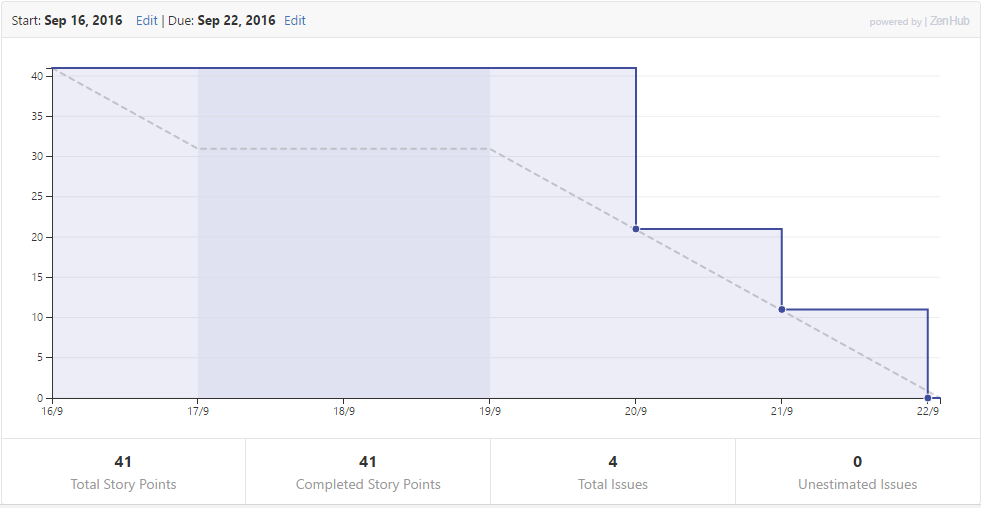
\includegraphics[width=0.99\textwidth]{Semana1}
\caption{Burndown de la semana 1}
\label{fig:A.2.1}
\end{figure}

\subsection{Sprint 2 (22/9/2016 - 30/9/2016)}
En la semana dos vamos a abarcar puntos de la interfaz y puntos de la documentación del proyecto y las tareas son:
 
\begin{itemize}
\item Documentación. 
\begin{itemize}
	\item Aspectos relevantes. 
	\item Técnicas y herramientas.
	\item Planificación temporal.
	\end{itemize}
\item Listas en la interfaz gráfica (Usar tablas para mostrar las rectas que hemos añadido manualmente).
\item Cargar imágenes con el file chooser.
\end{itemize}

\subsubsection{Cumplido:}
Hemos cumplido los objetivos aunque mas adelante y después de una revisión seguramente tengamos que modificar algunas cosas, añadir mas documentación ya que es la primera semana de documentación del proyecto.

Respecto al punto de la tabla donde aparezcan las listas de líneas que vamos añadiendo queda preguntar, si vendría bien añadir tres botones mas al modo manual.

Cosa que en la reunión con el Cliente (Rebeca) voy a exponer y posteriormente si parece bien desarrollar.

En cuanto al punto de cargar las imágenes con un \textit{file chooser} de paso, como me sobró algo de tiempo añadí una pantalla de inicio con un mensaje, así la primera vez que abramos la herramienta no se muestren tablas vacías ni una imagen predefinida.

Opte por hacer usar una pagina de inicio a modo de fachada y cuando se cargue la imagen ya iniciar todas las funcionalidades de la aplicación.
Gráfico del sprint 2 \ref{fig:A.2.2}.
\begin{figure}[h]
\centering
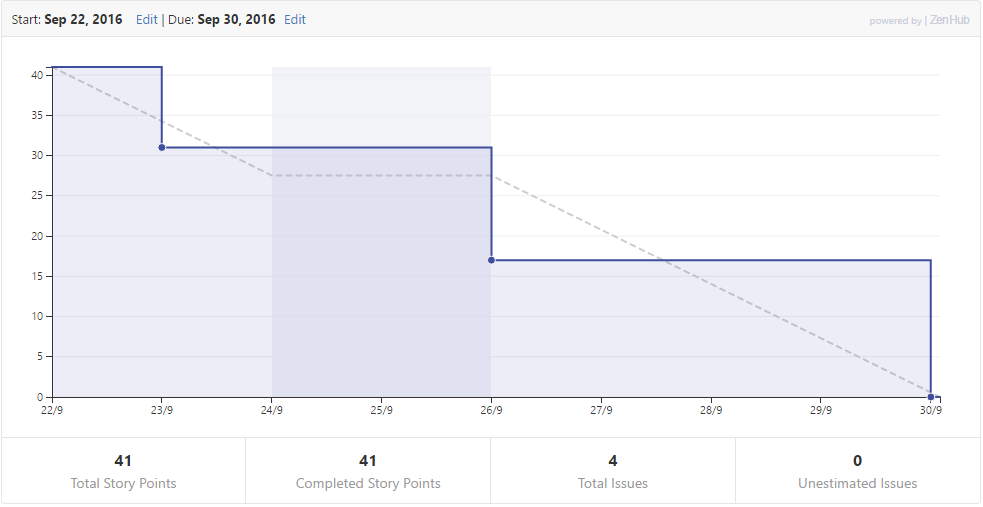
\includegraphics[width=0.99\textwidth]{Semana2}
\caption{Burndown de la semana 2}
\label{fig:A.2.2}
\end{figure}

\subsection{Sprint 3 (30/9/2016 - 7/10/2016)}
En la semana tres vamos a abarcar puntos de la interfaz GUI , generar el informe, y pasar actualizar  el código de PyQt4 a PyQt5 y las tareas son:

\begin{itemize}
	\item Acabar la GUI.
		\begin{itemize}
			\item Mostrar todas las líneas en la tabla.
			\item Poder borrar la línea seleccionada.
		\end{itemize} 
	\item Informe.
		\begin{itemize}
			\item Calcular estadísticas.
			\item Mirar documentación Python.
		\end{itemize}
	\item Pasar código de PyQt4 a PyQt5.
\end{itemize}
\subsubsection{Cumplido:}
Hemos cumplido los objetivos de esta semana y hemos generado funcionalidad a la tabla para agregar las líneas, también añadido que se ilumine la línea seleccionada dentro de la imagen en color amarillo. Hemos añadido funcionalidad para borrar la línea que tenemos seleccionada y también para poder limpiar la tabla completa.

Respecto a la tarea del informe, hemos calculado los estadísticos de todas las líneas, también su clasificación y escritura dentro de un fichero CSV, también la generación de una tabla latex que se actualiza a cada ejecución con los datos que han salido para poder pegarla fácilmente a un informe.

Como nos dimos cuenta que la versión de PyQt se había actualizado de la cuatro a la cinco pues hemos pasado el código a la nueva version y no ha sido muy difícil.

Gráfico del sprint 3 \ref{fig:A.2.3}.
\begin{figure}[h]
\centering
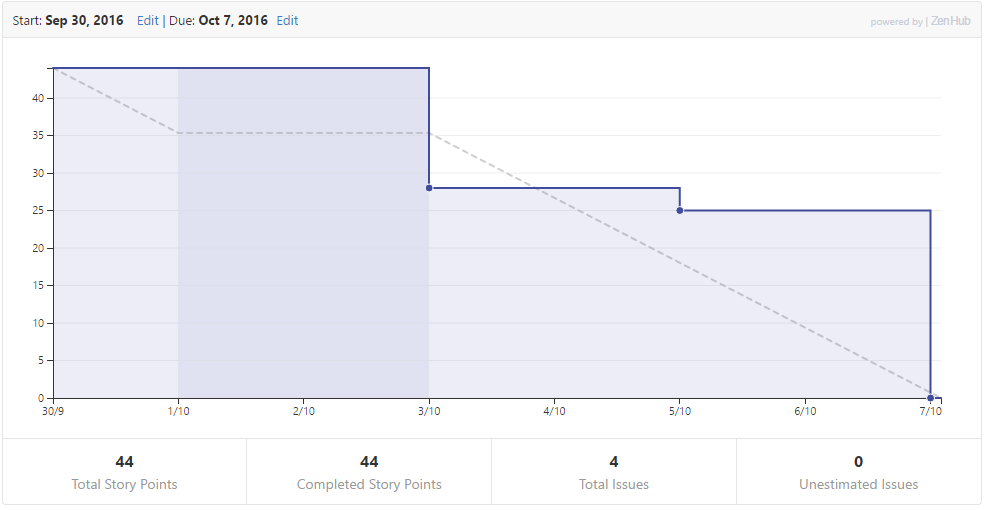
\includegraphics[width=0.99\textwidth]{Semana3}
\caption{Burndown de la semana 3}
\label{fig:A.2.3}
\end{figure}


\subsection{Sprint 4 (7/10/2016 - 14/10/2016)}
En esta semana vamos a abarcar el diseño software de la aplicación así como sacarlo de los NoteBooks y pasarlo a un IDE en condiciones con su subdivisión en clases y paquetes y las tareas son:
\begin{itemize}
	\item Diseño de la aplicación.
		\begin{itemize}
			\item Diagrama de clases.
			\item Diagrama de paquetes.
		\end{itemize}
		
	\item Implementación del código.
		
	\item Corrección de las memorias.
	
	\item Herramienta SonarQube.
	\begin{itemize}
		\item Ejecutar la aplicación.
		\item Corregir las horas de débito.
	\end{itemize}
\end{itemize}
\subsubsection{Cumplido:}
Hemos cumplido los objetivos de la semana.
En paralelo hemos implementado el diseño y el código a medida que teníamos una parte del diseño, de forma incremental, por lo que no se queda del todo reflejado cuando cerramos las tareas.\\

Hemos elegido Eclipse como IDE junto con su plugin PyDev para Python.

La división en clases hemos conseguido tener una primera estimación de como estaba la aplicación.
Respecto a la herramienta SonarQube hemos corregido todos los errores y defectos que salían, a mencionar que no había código repetido ni errores graves.

También detectamos un Bug y fue corregido.

Gráfico del sprint 4 \ref{fig:A.2.4}.
\begin{figure}[h]
\centering
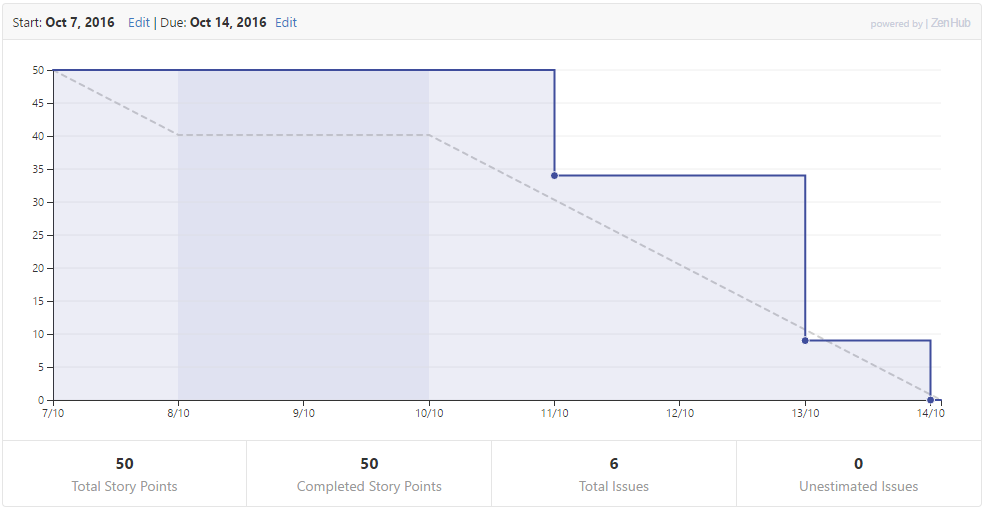
\includegraphics[width=0.99\textwidth]{Semana4}
\caption{Burndown de la semana 4}
\label{fig:A.2.4}
\end{figure}

\subsection{Sprint 5 (13/10/2016 - 22/10/2016)}
Esta semana vamos a continuar con el diseño de la aplicación aplicar los patrones correspondientes y paquetes de las clases.

\begin{itemize}
	\item Aplicar patrones de diseño
	\begin{itemize}
		\item Fachada.
		\item Mediador.
		\item Comando.
	\end{itemize}
	\item Documentar sobre los patrones usados.
	\item XML mirar documentación sobre ello.
\end{itemize}
\subsubsection{Cumplido:}
Esta semana, hemos cumplido con los objetivos, hemos documentado los patrones y decidido que con el mediador ya nos servia y el fachada como entrada a la aplicación.
 
El patrón comando en Python no le hemos visto mucho sentido ya que en Python el connect con la función se hace en una sola linea por lo que no hace falta utilizar un patrón comando.

Respecto al XML hemos mirado documentación y lo hemos implementado que guarde los nombres de todos los archivos que generan un proyecto.

Gráfico del sprint 5 \ref{fig:A.2.5}.

\begin{figure}[h]
\centering
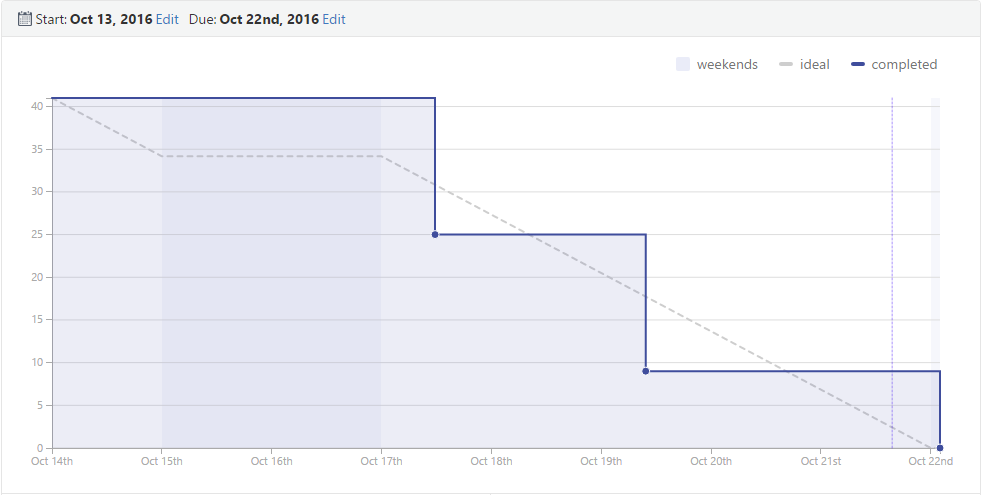
\includegraphics[width=0.99\textwidth]{Semana5}
\caption{Burndown de la semana 5}
\label{fig:A.2.5}
\end{figure}
\subsection{Sprint 6 (22/10/2016 - 28/10/2016)}
Esta semana vamos a intentar ir terminando las tareas para poder la semana que viene tener un prototipo entregable de la aplicación.

\begin{itemize}
\item Completar menús de la GUI.
	\begin{itemize}
		\item Guardar.
		\item Cargar.
		\item Acerca de.
		\item Ayuda.
	\end{itemize}
\item Completar documentación de los fuentes.
	\begin{itemize}
		\item Paquete código.
		\item Paquete gui.
	\end{itemize}
\item Pruebas unitarias.
	\begin{itemize}
		\item Teses paquete código.
		\item Teses paquete gui.
	\end{itemize}
\end{itemize}
\subsubsection{Cumplido:}
Esta semana, hemos cumplido con los objetivos, aunque en el gráfico no queda reflejado por el ataque del día 21 de octubre de 2016 \url{https://es.wikipedia.org/wiki/Ciberataque_a_Dyn_de_octubre_de_2016} no pude cerrar las tareas del anterior sprint ni crear las de este.
Respecto a los menús de la gui, hemos añadido y renombrado los campos.

Las funcionalidades añadidas son que guardemos los cambios, podamos abrir y modificar un proyecto, el acerca de y el botón sobre el que va a colgar la ayuda.
También hemos documentado los métodos de las clases del código fuente Python para poder generar la documentación automática con PyDoc.

También hemos desarrollado las pruebas unitarias de la aplicación de todas aquellas funciones que se podía comprobar. 


Gráfico del sprint 6 \ref{fig:A.2.6}.
\begin{figure}[h]
\centering
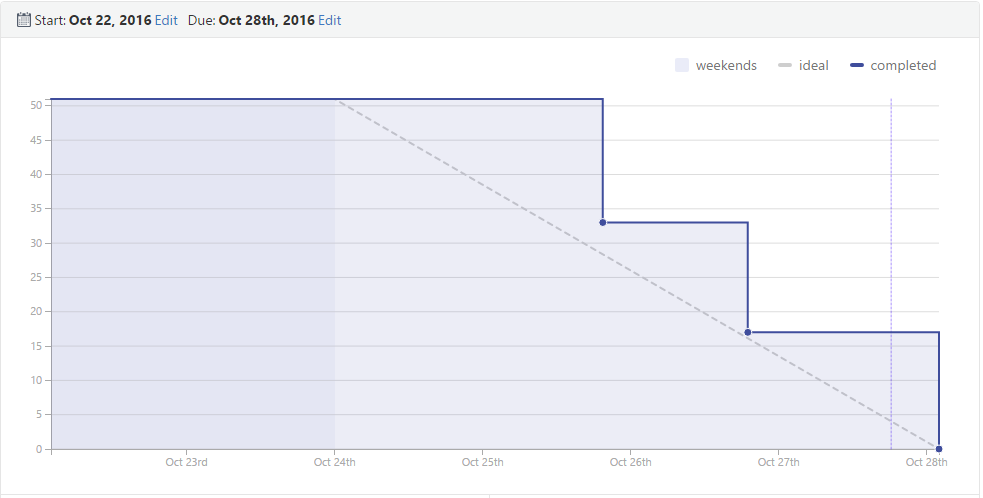
\includegraphics[width=0.99\textwidth]{Semana6}
\caption{Burndown de la semana 6}
\label{fig:A.2.6}
\end{figure}

\subsection{Sprint 7 (13/10/2016 - 22/10/2016)}

\section{Estudio de viabilidad}

\subsection{Viabilidad económica}

\subsection{Viabilidad legal}


